\documentclass{ximera}
\usepackage{tikz}
\usepackage{color}
\usepackage{amsmath,amssymb,amsfonts}
\usepackage{graphicx}
%\usepackage{helvet}
%\renewcommand{\familydefault}{\sfdefault}
\author{Jeffrey Kuan}
\input{../preamble} %% Loads the graphics path
\title{An example webpage}
\license{CC: 0}
\begin{document}

\begin{abstract}
   I like Taylor Swift.
\end{abstract}
\maketitle
%\part{Introduction}
%\chapterstyle
%    \activity{basics/basicWorksheet}
%    \sectionstyle
%    \activity{basics/exercises/someExercises}

%    \chapterstyle
%    \activity{basics/graphicsInteractives}

Accessibility statement: This webpage is WCAG2.1AA compliant, and I tested out this webpage on NVDA. 
You can also \href{https://ximera.osu.edu/firststeps24html/aFirstStepInXimera/basics/MAA_AMS_Example.tex}{download the TeX source file.}

\section{About this webpage}
This webpage was created with \href{https://ximera.osu.edu/}{Ximera}, an 
interactive textbook platform hosted by Ohio State University. The Ximera Project is funded 2024-2026 (with no other external funding) by a 
\$2,125,000 \href{https://www.ed.gov/grants-and-programs/grants-higher-education/improvement-postsecondary-education/open-textbooks-pilot-program}{Open Textbooks Pilot Program} grant from the federal Department of Education.



\section{An example of alternative text}
Whenever I get to this part of ``Folklore: The Long Pond Studio Sessions'' \cite{F:LPSS} 

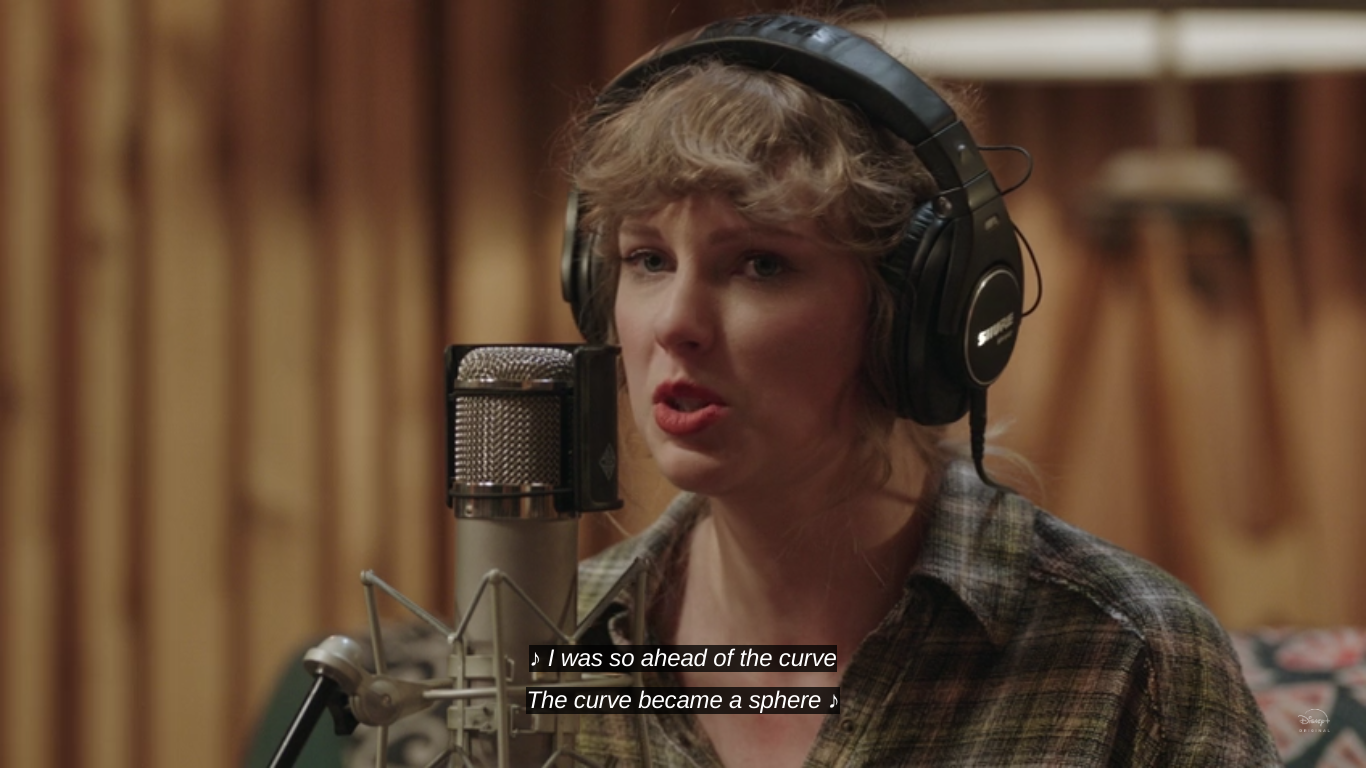
\includegraphics[scale=0.5,alt="Taylor Swift in front of a microphone wearing headphones. There are the captions 'I was so ahead of the curve, the curve became a sphere.'"]{TaylorSwiftScreenshot.png}

from ``This Is Me Trying'' \cite{TS8}, I think about math. 


\begin{thebibliography}{10}

\bibitem[TS8]{TS8} Swift, Taylor: “This Is Me Trying.” Folklore, Republic Records, 2020.

\bibitem[F:LPSS]{F:LPSS} Swift, Taylor: "Folklore: The Long Pond Studio Sessions." Taylor Swift Productions, 2020. 

\end{thebibliography}

\end{document}